\section{Maschine Learning}

Der Fokus dieser Arbeit ist die Ermitellung von Design von Quellcode durch die Anwendung von Maschine Learning.
Dieser Teil der Arbeit ist für die Erläuterung von verwendeten Metriken, angewandeten Techniken und ausgewählter Klasszifizierer geweidment.

% TODO: \subsection{Terminologie} falls notwendig
\subsection{Metriken für Evaluierung von Modellen}

Um die Leistung eines Klasszifierers zu ermitelln, bedarf es einer Menge an Metriken, womit beurteilt werden, ob der Klassfizierer wie erwartet performt.
In Kontext dieser Aussage wird in der Domäne des Maschine Learnings bekannte Metriken aus dem Bereich der Statistik angewendet.
In diesem Abschnitt wird eine Auswahl von solchen Metriken erkläutert, die in der Literaturrecherche als auch in den Sektionen der Methodik und Implementierung erwähnt werden.
Für die Ermittelung der Metriken werden folgende Größen definiert:

\begin{description}
    \item TP (True Positive): Anzahl echt postiver Klassifizierungen
    \item TN (True Negative): Anzahl echt negativer Klassifizierungen
    \item FP (False Postive): Anzahl falsch positiv Klassifizierungen
    \item FN (False Negative): Anzahl falsch negativ Klassifizierungen
\end{description}

Anhand dieser Größen werden folgende Metriken definiert:

\begin{description}
    \item \textit{Accuracy (Genauigkeit)}: Dieser Wert gibt an, wie das Verhältnis zwischen den klassifizierten Beobachtungen zur Gesamtzahl der Beobachtungen ist.
    \\
    \\
    $Accuracy = \frac{\text{Anzahl der korrekten Vorhersagen}}{\text{Gesamtzahl der Vorhersagen}} = \frac{TP+TN}{TP+TN+FP+FN}$

    \item \textit{Precision (Präzision)}: Dieser Wert gibt das Verhältnis an, wie die korrekt positiv klassifizierten Beobachtungen zur Gesamtzahl der als positiv klassifizierten Beobachtungen stehen.
    \\
    \\
    $Precision = \frac{TP}{TP+FP}$

    \item \textit{Recall (Sensitivität)}: : Dies ist das Verhältnis der positiv klassifizierten Beobachtungen zur Gesamtzahl der tatsächlichen positiven Beobachtungen.
    \\
    \\
    $Recall = \frac{TP}{TP+FN}$
    
    \item \textit{ F1-Score}: Der F1-Score ist das harmonische Mittel von Präzision und Recall und gibt ein besseres Maß für die unbalancierten Klassen als die Genauigkeit allein.
    \\
    \\
    $\textit{\text{F1-Score}} = 2 * \frac{Precision * Recall}{Precision + Recall} = \frac{2*TP}{2*TP + FP + FN}$
\end{description}

\pagebreak

\subsection{Validierung und Optimierung von Modellen}

Neben dem Zusammentragen von relevanten Datenpukten für die Erhebung eines geeigneten Datensatzes ist das Validierung und Optimierung des Maschine Learning Modells eines der relevanten Schritte im gesammten Prozess, 
um damit das Modell dessen Aufgabe möglichst zufriendenstellend erfülllen kann. 
In diesem Teil der Arbeit werden Techniken bzw. Methoden erläutert, die in der Validierungs- oder Optimierungsphase angewendet werden können.


\subsubsection*{Kreuzvalidierung von Modellen}
Nach dem Tranieren des Modells für einen Datensatz ist von Interesse, wie das Modell neue unbekannte Datenpunkte umgeht und diese Leistung anhand einer Metrik zu messen.
Dies stellt den Kernpunkt der Validierungsphase dar. Ein naiver Ansatz, die gleiche Menge an Datenpunkten zu verwenden, worauf das Modell in der Trainingsphase traniert wurde.
Dabei ist jeder Datenpunkt des Datensatzes dem Modell bereits bekannt, wodurch es nicht auf wirklich unbekannte Datenpunkte validiert.
Eine Möglichkeit dem entgegenzukommen ist das Aufteilen des Datensatzes in Trainings- und Validationsdatensatz, wobei meist der Trainingsdatensatz den größere Menge an Datennpunkten zugesprochen wird.
Jedoch besteht hier der Nachteil, das in der Trainingsphase die Datenpunkte in dem Validierungsdatensatz wegfallen.
Um diesen Nachteil zu negieren, kann die Technik der Cross Validation oder Kreuzvalidierung angewendet werden.

Hierbei wird zunächst eine natürliche Zahl \textit{n} bestimmt, die angibt, in wie viele gleich große Teil der Datensatz aufgespaltet wird.
Die Trainings- und Validierungsphase wird hierbei zu einem Schritt zusammengefasst und das Modell wird iterativ \textit{n}-Mal traniert und anhand der betimmten Metrik evaluiert.

\begin{figure}[h]
    \centering
    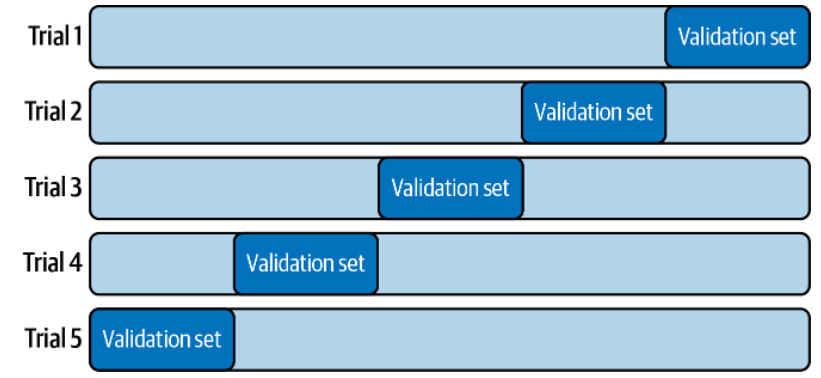
\includegraphics[scale=0.5]{figures/cross_validation}
    \caption{Kreuzvalidierung mit \textit{n} = 5}
    \label{fig:cross_validation}
\end{figure}
Wie aus Abbildung \ref{fig:cross_validation} zu entnehmen ist, wird in der \textit{i}-ten Iteration das $k-i$-te Sektion des Datensatzes für die Validierung und restlichen
für das Training des Modells verwendet. Das Resultat dieser Operation ist abhängig von Implementierung der Kreuzvalidierung die Iteration des Modells mit der besten Evaluation und eine Liste von Werten, die Leistung des Modells in der jeweiligen Iteration angibt.

%%TODO: Add citiations from book
\subsection{Betrachete Klasszifizierer}